\begin{figure}[t]
    \vspace*{15pt}
    \centering
    % \begin{tabular}{c@{\hspace{1.5pt}}c@{\hspace{1.5pt}}}
    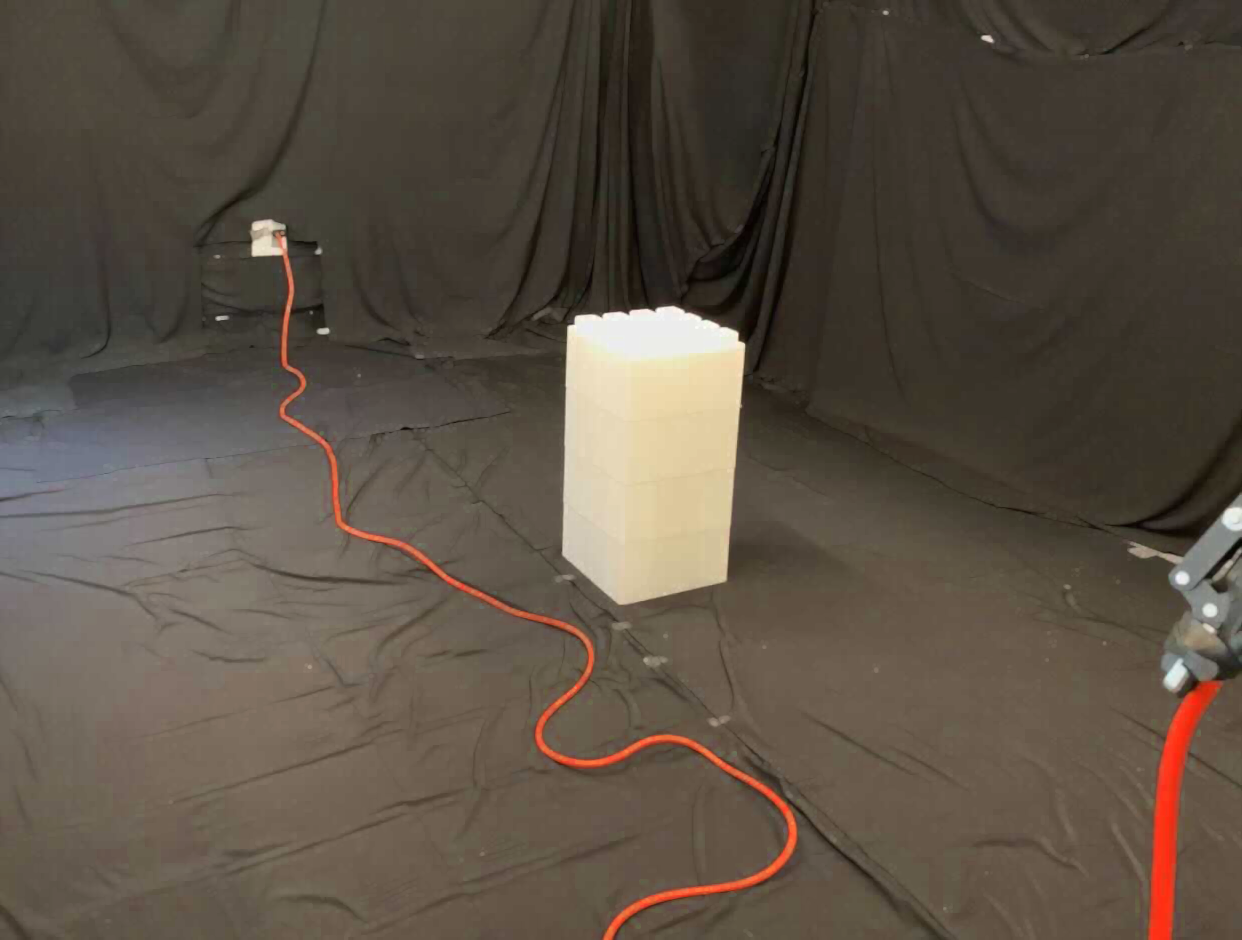
\includegraphics[width=120pt]{figures/failure_b4.png}\hfill
    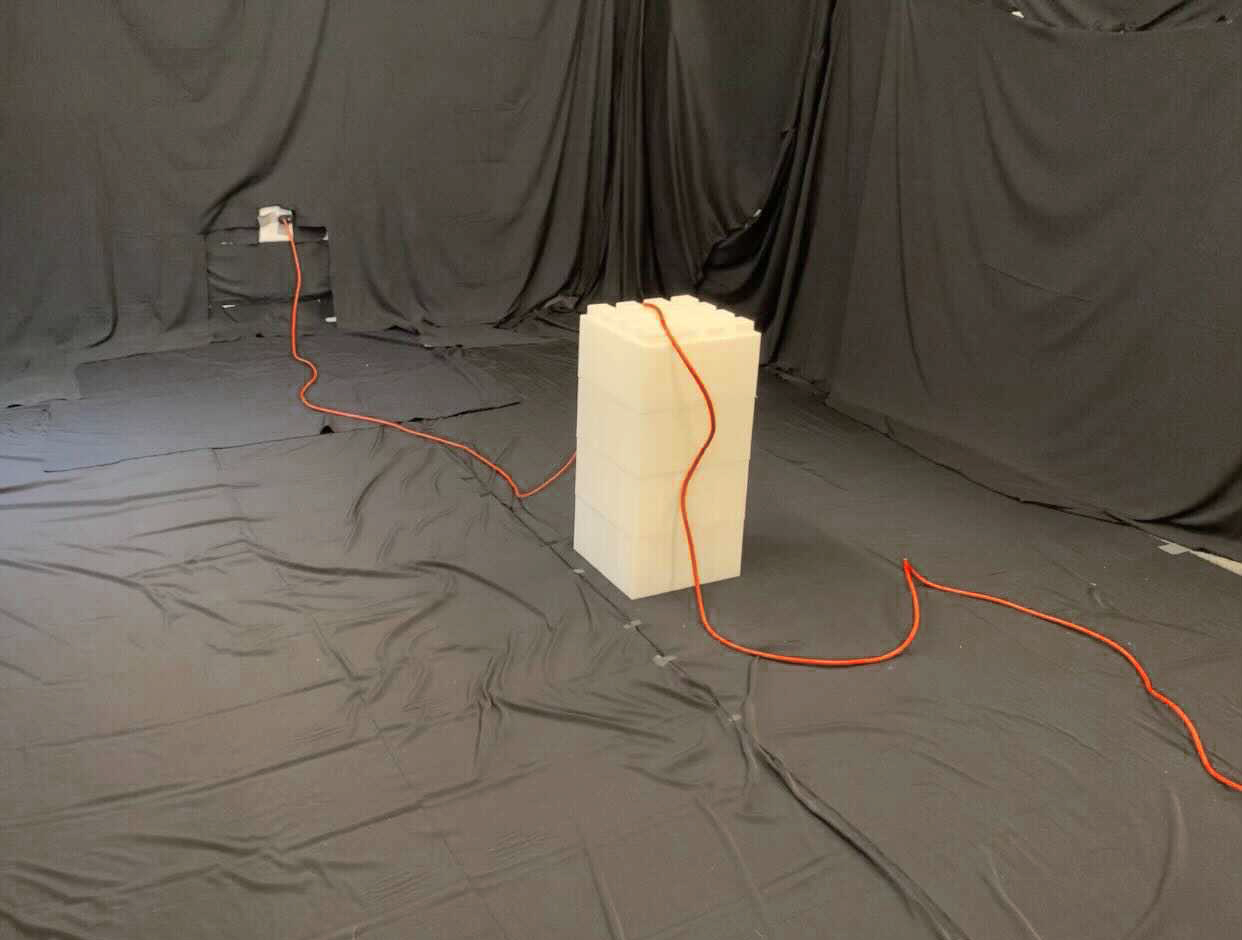
\includegraphics[width=120pt]{figures/failure_2.png}
    % \end{tabular}
    \caption{\textbf{Failure mode}. The 16-gauge 6.2~m orange cable is too long for the vaulting motion.  \textbf{Left:} before the motion there is too much slack. \textbf{Right:} the vaulting motion that works for shorter cables does not clear the obstacle.} %and the resulting cable terminal configuration is not on the other side (right) of the obstacle, and instead the cable lands on the obstacle.}
    
    \label{fig:failure}
\end{figure}